\documentclass[11pt,oneside]{book}
\usepackage[utf8]{inputenc}
\usepackage[T1]{fontenc}
\usepackage{charter}
\usepackage{courier}
\usepackage[scaled=0.92]{helvet}
\usepackage{microtype}
\usepackage{geometry}
\geometry{
  letterpaper,
  left=1.1in,
  right=1.1in,
  top=1.0in,
  bottom=1.0in,
  headheight=24pt
}

\usepackage{amsmath,amssymb}
\usepackage{booktabs}
\usepackage{graphicx}
\usepackage{xcolor}
\usepackage{fancyhdr}
\usepackage{titlesec}
\usepackage{enumitem}
\usepackage{listings}
\usepackage{tcolorbox}
\tcbuselibrary{skins,breakable}
\usepackage{tikz}
\usetikzlibrary{arrows.meta,positioning,shapes.geometric,calc,decorations.pathreplacing,fit}

% Color Palette - Manning / O'Reilly inspired muted functional palette
\definecolor{textdark}{RGB}{30, 41, 59}       % Deep slate text
\definecolor{headingblue}{RGB}{15, 23, 42}    % Slate 900
\definecolor{codebg}{RGB}{248, 250, 252}       % Slate 50 background
\definecolor{codeframe}{RGB}{226, 232, 240}   % Slate 200 border
\definecolor{linkblue}{RGB}{2, 132, 199}      % Sky 600

% Callout colors
\definecolor{intuitionTeal}{RGB}{13, 148, 136}
\definecolor{intuitionBg}{RGB}{240, 253, 250}
\definecolor{hoodSlate}{RGB}{71, 85, 105}
\definecolor{hoodBg}{RGB}{248, 250, 252}
\definecolor{exampleBlue}{RGB}{37, 99, 235}
\definecolor{exampleBg}{RGB}{239, 246, 255}
\definecolor{mistakeAmber}{RGB}{217, 119, 6}
\definecolor{mistakeBg}{RGB}{254, 252, 232}
\definecolor{warningRed}{RGB}{220, 38, 38}
\definecolor{warningBg}{RGB}{254, 242, 242}
\definecolor{tryViolet}{RGB}{124, 58, 237}
\definecolor{tryBg}{RGB}{245, 243, 255}

% Typography & Spacing
\linespread{1.14}
\setlength{\parindent}{0pt}
\setlength{\parskip}{7pt plus 2pt minus 1pt}

% Section Titles Styling (Modern & Proportionate)
\titleformat{\chapter}[display]
  {\normalfont\sffamily\bfseries\color{headingblue}}
  {\vspace{-20pt}\flushleft\normalsize\scshape\color{gray}CHAPTER \thechapter}
  {6pt}
  {\huge\raggedright}[\vspace{10pt}\hrule height 0.8pt\vspace{14pt}]
\titlespacing*{\chapter}{0pt}{10pt}{20pt}

\titleformat{\section}
  {\normalfont\sffamily\Large\bfseries\color{headingblue}}
  {\thesection}{1em}{}
\titlespacing*{\section}{0pt}{16pt plus 3pt minus 2pt}{6pt}

\titleformat{\subsection}
  {\normalfont\sffamily\large\bfseries\color{headingblue}}
  {\thesubsection}{1em}{}
\titlespacing*{\subsection}{0pt}{12pt plus 2pt minus 2pt}{4pt}

\titleformat{\subsubsection}
  {\normalfont\sffamily\normalsize\bfseries\color{headingblue}}
  {\thesubsubsection}{1em}{}
\titlespacing*{\subsubsection}{0pt}{10pt plus 2pt minus 1pt}{3pt}

% Header & Footer
\pagestyle{fancy}
\fancyhf{}
\fancyhead[L]{\small\sffamily\color{gray}\nouppercase{\leftmark}}
\fancyhead[R]{\small\sffamily\bfseries\thepage}
\renewcommand{\headrulewidth}{0.4pt}
\renewcommand{\headrule}{\hbox to\headwidth{\color{gray!30}\leaders\hrule height \headrulewidth\hfill}}
\fancypagestyle{plain}{
  \fancyhf{}
  \fancyfoot[C]{\small\sffamily\thepage}
  \renewcommand{\headrulewidth}{0pt}
}

% Code Listings Styling
\lstset{
  backgroundcolor=\color{codebg},
  basicstyle=\ttfamily\footnotesize\color{textdark},
  breakatwhitespace=false,
  breaklines=true,
  captionpos=b,
  commentstyle=\color{gray!80!black}\itshape,
  frame=single,
  rulecolor=\color{codeframe},
  framerule=0.6pt,
  keepspaces=true,
  keywordstyle=\bfseries\color{blue!80!black},
  stringstyle=\color{green!50!black},
  numbers=left,
  numbersep=8pt,
  numberstyle=\tiny\color{gray!70},
  showspaces=false,
  showstringspaces=false,
  showtabs=false,
  tabsize=2,
  xleftmargin=12pt,
  framexleftmargin=10pt,
  framexrightmargin=4pt,
  framextopmargin=4pt,
  framexbottommargin=4pt
}

% 6 Pedagogical Callout Boxes (Muted, Left-Border Styling)
\newtcolorbox{intuitionbox}[1][]{
  enhanced,
  breakable,
  colback=intuitionBg,
  colframe=intuitionTeal,
  arc=1pt,
  boxrule=0pt,
  leftrule=3.5pt,
  top=6pt,bottom=6pt,left=10pt,right=10pt,
  coltitle=intuitionTeal,
  fonttitle=\sffamily\bfseries\small,
  title={Intuition \ifstrempty{#1}{}{: #1}},
  attach title to upper=\par\vspace{4pt}
}

\newtcolorbox{underthehoodbox}[1][]{
  enhanced,
  breakable,
  colback=hoodBg,
  colframe=hoodSlate,
  arc=1pt,
  boxrule=0pt,
  leftrule=3.5pt,
  top=6pt,bottom=6pt,left=10pt,right=10pt,
  coltitle=hoodSlate,
  fonttitle=\sffamily\bfseries\small,
  title={Under the Hood \ifstrempty{#1}{}{: #1}},
  attach title to upper=\par\vspace{4pt}
}

\newtcolorbox{realworldbox}[1][]{
  enhanced,
  breakable,
  colback=exampleBg,
  colframe=exampleBlue,
  arc=1pt,
  boxrule=0pt,
  leftrule=3.5pt,
  top=6pt,bottom=6pt,left=10pt,right=10pt,
  coltitle=exampleBlue,
  fonttitle=\sffamily\bfseries\small,
  title={Real-World Scenario \ifstrempty{#1}{}{: #1}},
  attach title to upper=\par\vspace{4pt}
}

\newtcolorbox{commonmistakebox}[1][]{
  enhanced,
  breakable,
  colback=mistakeBg,
  colframe=mistakeAmber,
  arc=1pt,
  boxrule=0pt,
  leftrule=3.5pt,
  top=6pt,bottom=6pt,left=10pt,right=10pt,
  coltitle=mistakeAmber,
  fonttitle=\sffamily\bfseries\small,
  title={Common Mistake \ifstrempty{#1}{}{: #1}},
  attach title to upper=\par\vspace{4pt}
}

\newtcolorbox{productionwarningbox}[1][]{
  enhanced,
  breakable,
  colback=warningBg,
  colframe=warningRed,
  arc=1pt,
  boxrule=0pt,
  leftrule=3.5pt,
  top=6pt,bottom=6pt,left=10pt,right=10pt,
  coltitle=warningRed,
  fonttitle=\sffamily\bfseries\small,
  title={Production Warning \ifstrempty{#1}{}{: #1}},
  attach title to upper=\par\vspace{4pt}
}

\newtcolorbox{tryityourselfbox}[1][]{
  enhanced,
  breakable,
  colback=tryBg,
  colframe=tryViolet,
  arc=1pt,
  boxrule=0pt,
  leftrule=3.5pt,
  top=6pt,bottom=6pt,left=10pt,right=10pt,
  coltitle=tryViolet,
  fonttitle=\sffamily\bfseries\small,
  title={Try It Yourself \ifstrempty{#1}{}{: #1}},
  attach title to upper=\par\vspace{4pt}
}

% Chapter Goals / Roadmaps Box
\newtcolorbox{chaptergoalsbox}{
  enhanced,
  breakable,
  colback=gray!4!white,
  colframe=gray!40!white,
  arc=2pt,
  boxrule=0.8pt,
  top=8pt,bottom=8pt,left=12pt,right=12pt,
  coltitle=headingblue,
  fonttitle=\sffamily\bfseries\small,
  title={Roadmap \& Prerequisites},
  attach title to upper=\par\vspace{4pt}
}

% Hyperref setup (Muted, readable links)
\usepackage[
  colorlinks=true,
  linkcolor=headingblue,
  citecolor=linkblue,
  urlcolor=linkblue,
  bookmarksnumbered=true,
  pdfstartview=FitH
]{hyperref}


\begin{document}
\frontmatter
\pagestyle{empty}

\begin{center}
  \vspace*{2cm}
  {\Huge\sffamily\bfseries\color{headingblue} Modern Engineering Curriculum}\\[12pt]
  {\Large\sffamily\color{gray} A Structured Self-Study Roadmap Across 5 Engineering Volumes}\\[30pt]
  \hrule height 1.2pt
  \vspace*{25pt}
  {\normalsize\sffamily Designed for Deep Technical Understanding, Job Readiness, and Production Mastery}
\end{center}

\vspace{3cm}

\begin{tcolorbox}[
  enhanced,
  colback=white,
  colframe=gray!30!white,
  boxrule=0.8pt,
  arc=2pt,
  left=15pt,right=15pt,top=12pt,bottom=12pt
]
\sffamily\small
\textbf{How to Use This Roadmap:}
\begin{itemize}[leftmargin=15pt]
  \item \textbf{Track A (Immediate Job Readiness -- Modern PHP \& Web Integrations):} Complete Volume I (Chapters 1--7) and Projects 1, 2, 3. Focus heavily on PHP-FPM execution, memory semantics (zvals, CoW), PDO transactions, and webhook signature verification with replay defense.
  \item \textbf{Track B (Cloud Infrastructure \& DevSecOps):} Volume III (Chapters 1--7) alongside Projects 8, 9, 10. Learn Linux namespaces, Docker/Kubernetes internals, and Terraform DAG execution.
  \item \textbf{Track C (AI Engineering \& Systems):} Volume II (Chapters 1--7) alongside Projects 5, 6, 7. Learn LangGraph state machines, HNSW vector search, hybrid retrieval, and LLM evaluation pipelines.
  \item \textbf{Track D (Distributed Systems \& Architecture):} Volume IV \& Volume V (all chapters) alongside Projects 11, 12. Master CAP/PACELC, Raft consensus, Transactional Outbox, Sagas, C4 modeling, and AI inference economics.
\end{itemize}
\end{tcolorbox}

\newpage
\pagestyle{fancy}
\mainmatter

\chapter*{Curriculum Dependency Map}

The five volumes form a cohesive engineering continuum. The diagram below illustrates how core concepts build progressively upon lower-level foundations.

\begin{figure}[htbp]
\centering
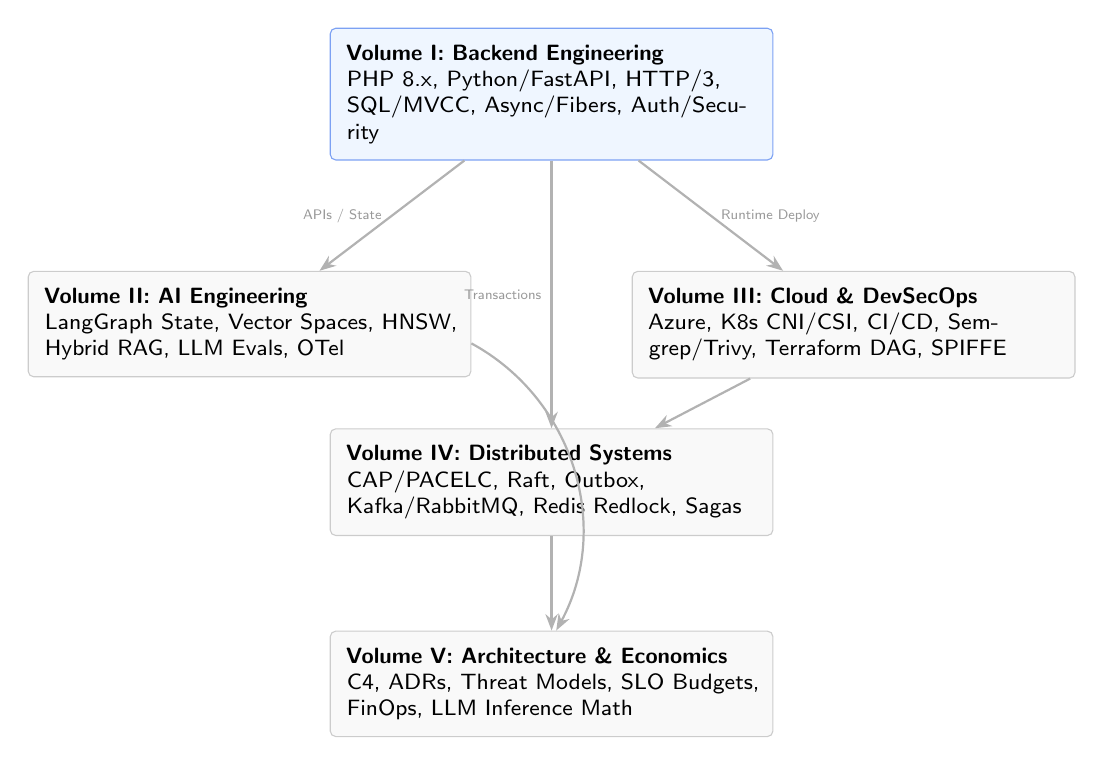
\begin{tikzpicture}[
  node distance=1.2cm and 0.8cm,
  block/.style={rectangle, draw=gray!40, fill=gray!5, rounded corners=2pt, text width=5.2cm, minimum height=1.1cm, align=left, inner sep=6pt, font=\sffamily\footnotesize},
  highlight/.style={rectangle, draw=exampleBlue!60, fill=exampleBg, rounded corners=2pt, text width=5.2cm, minimum height=1.1cm, align=left, inner sep=6pt, font=\sffamily\footnotesize},
  arrow/.style={-{Stealth[scale=0.9]}, thick, color=gray!60}
]

% Nodes
\node[highlight] (v1) {\textbf{Volume I: Backend Engineering}\\PHP 8.x, Python/FastAPI, HTTP/3, SQL/MVCC, Async/Fibers, Auth/Security};
\node[block, below left=1.4cm and -1.8cm of v1] (v2) {\textbf{Volume II: AI Engineering}\\LangGraph State, Vector Spaces, HNSW, Hybrid RAG, LLM Evals, OTel};
\node[block, below right=1.4cm and -1.8cm of v1] (v3) {\textbf{Volume III: Cloud \& DevSecOps}\\Azure, K8s CNI/CSI, CI/CD, Semgrep/Trivy, Terraform DAG, SPIFFE};
\node[block, below=3.4cm of v1] (v4) {\textbf{Volume IV: Distributed Systems}\\CAP/PACELC, Raft, Outbox, Kafka/RabbitMQ, Redis Redlock, Sagas};
\node[block, below=1.2cm of v4] (v5) {\textbf{Volume V: Architecture \& Economics}\\C4, ADRs, Threat Models, SLO Budgets, FinOps, LLM Inference Math};

% Arrows
\draw[arrow] (v1) -- node[left, font=\tiny\sffamily, color=gray!80]{APIs / State} (v2);
\draw[arrow] (v1) -- node[right, font=\tiny\sffamily, color=gray!80]{Runtime Deploy} (v3);
\draw[arrow] (v1) -- node[left, font=\tiny\sffamily, color=gray!80]{Transactions} (v4);
\draw[arrow] (v3) -- (v4);
\draw[arrow] (v4) -- (v5);
\draw[arrow] (v2) to [bend left=45] (v5);

\end{tikzpicture}
\caption{Curriculum Architecture and Prerequisite Flow}
\end{figure}

\section*{Detailed Volume \& Chapter Breakdown}

\subsection*{Volume I: Backend Engineering (7 Chapters)}
\begin{enumerate}[leftmargin=18pt]
  \item \textbf{Modern PHP Engineering}: PHP-FPM, Zend Engine, OPcache, JIT, type system, zvals, memory management, closures, webhooks, idempotency.
  \item \textbf{Python and FastAPI}: CPython, bytecode, GIL, asyncio event loop, epoll/kqueue, ASGI, Pydantic v2, dependency injection.
  \item \textbf{Backend Architecture, HTTP and APIs}: HTTP/1.1 vs HTTP/2 vs HTTP/3 (QUIC), REST, WebSockets, SSE, gRPC.
  \item \textbf{Databases, SQL and ORM Design}: PostgreSQL engine, WAL, page storage, B-Trees, MVCC, isolation levels, row locking, query plans.
  \item \textbf{Asynchronous Programming and Concurrency}: Cooperative vs preemptive multitasking, threads vs fibers, CSP channels, Revolt/Amp.
  \item \textbf{Authentication, Authorization and Security}: Passwords (Argon2id), sessions, JWT security, OAuth 2.0 PKCE, RBAC/ABAC, OWASP top 10.
  \item \textbf{Testing and Production Reliability}: Testing pyramid, mutation testing, Testcontainers, circuit breakers, rate limiting.
\end{enumerate}

\subsection*{Volume II: AI Engineering (7 Chapters)}
\begin{enumerate}[leftmargin=18pt]
  \item \textbf{LangGraph \& State Machines}: Pregel execution model, StateGraph, reducers, checkpointing, human-in-the-loop interrupts.
  \item \textbf{Production-Grade RAG}: Chunking trade-offs, lost-in-the-middle, parent-document retrieval, multi-vector indexing.
  \item \textbf{Embeddings and Vector Databases}: Vector space geometry, ANN search, HNSW graph construction, Qdrant/pgvector internals.
  \item \textbf{Retrieval Algorithms and Reranking}: BM25 sparse search, dense-sparse hybrid fusion (RRF), Cross-Encoder reranking.
  \item \textbf{Agent Architectures and Orchestration}: ReAct, Plan-and-Solve, Reflexion, tool calling schemas, supervisor-worker models.
  \item \textbf{LLM Evaluations}: Ragas/TruLens, Groundedness, Answer Relevance, Context Precision, synthetic test generation.
  \item \textbf{Observability and Tracing}: OpenTelemetry for AI, distributed spans, token and cost attribution, Langfuse.
\end{enumerate}

\subsection*{Volume III: Cloud Engineering and DevSecOps (7 Chapters)}
\begin{enumerate}[leftmargin=18pt]
  \item \textbf{Azure Fundamentals and Architecture}: Management hierarchy, VNets, NSGs, Private Endpoints, App Services, Container Apps.
  \item \textbf{Azure OpenAI and Azure AI Search}: Enterprise provisioning, PTU vs Pay-Go, content filters, semantic search, hybrid vector index.
  \item \textbf{Docker and Kubernetes Internals}: Linux namespaces, cgroups v2, containerd/runc, K8s control plane, kubelet, HPA, KEDA.
  \item \textbf{CI/CD Pipelines}: Runner security, GitHub Actions matrixing, Blue-Green deployments, Canary rollouts.
  \item \textbf{DevSecOps}: SAST (Semgrep), SCA (Trivy), secret scanning (TruffleHog), image signing (Cosign), SBOM (Syft).
  \item \textbf{Terraform and Infrastructure as Code}: HCL parser, DAG evaluation walk, state locking (Azure Blob leases), drift reconciliation.
  \item \textbf{Infrastructure Security}: Zero Trust, least privilege, mTLS with SPIFFE/SPIRE, Azure Key Vault secret rotation.
\end{enumerate}

\subsection*{Volume IV: Distributed Systems (9 Chapters)}
\begin{enumerate}[leftmargin=18pt]
  \item \textbf{Distributed Systems Fundamentals}: Physical limits, network latency, clock skew (NTP, TrueTime, Vector clocks), fault models.
  \item \textbf{CAP Theorem and Consistency Models}: PACELC theorem, Linearizability vs Eventual consistency, Raft consensus algorithm.
  \item \textbf{Transactions and Concurrency}: Two-Phase Commit (2PC), coordinator crash states, 3PC, distributed deadlocks.
  \item \textbf{Messaging Systems}: Delivery semantics (at-most-once, at-least-once, exactly-once), queues vs streams, DLQs.
  \item \textbf{Kafka and RabbitMQ Internals}: Kafka commit log, partitions, ISR replication, zero-copy read vs RabbitMQ AMQP exchanges.
  \item \textbf{Redis and Caching Topologies}: Redis event loop, skiplists, LRU/LFU, cache stampedes, Sentinel HA, Cluster hash slots.
  \item \textbf{Distributed Locking}: Mutex semantics, TTL leases, the Redlock debate (Kleppmann analysis), fencing tokens.
  \item \textbf{Sagas, CQRS and Event Sourcing}: Dual-write failure, Transactional Outbox pattern, CDC, Orchestrated Sagas, CQRS projections.
  \item \textbf{Reliability and Fault Tolerance}: Failure detectors, bulkheads, load shedding, retry storms with jitter, chaos engineering.
\end{enumerate}

\subsection*{Volume V: Software Architecture and Engineering Economics (9 Chapters)}
\begin{enumerate}[leftmargin=18pt]
  \item \textbf{C4 Architecture Modeling}: System Context, Container, Component, and Code diagrams.
  \item \textbf{UML and Sequence Diagrams}: Lifelines, synchronous/asynchronous flows, combined fragments, race condition modeling.
  \item \textbf{Technical Design Documents (TDD)}: Google/Uber RFC style documents, architecture specifications, operational readiness.
  \item \textbf{Architecture Decision Records (ADRs)}: Michael Nygard format, capturing context, decisions, trade-offs, and consequences.
  \item \textbf{Requirements Engineering}: Functional vs Non-Functional requirements (FURPS+), availability nines, latency percentiles.
  \item \textbf{Threat Modeling}: STRIDE methodology, Data Flow Diagrams (DFDs), trust boundaries, mitigation mapping.
  \item \textbf{SLOs, SLIs and SLAs}: Math for SLIs, error budget calculations, multi-window burn rate alerts, error budget freezes.
  \item \textbf{Cloud FinOps}: Inform, Optimize, Operate phases, cloud unit metrics, compute rightsizing, Reserved Instances.
  \item \textbf{AI Inference Economics and Cost Optimization}: GPU memory bandwidth limits, KV cache memory formulas, vLLM PagedAttention, speculative decoding.
\end{enumerate}

\section*{The 12 Practical Engineering Projects}
\begin{table}[htbp]
\centering\small
\begin{tabular}{lp{6.5cm}l}
\toprule
\textbf{Project} & \textbf{Title \& Description} & \textbf{Volume} \\
\midrule
\texttt{p01} & PHP 8.3 PDO E-Commerce Order Service with Transactions & Volume I \\
\texttt{p02} & Production Webhook Receiver (HMAC-SHA256, Replay, Idempotency) & Volume I \\
\texttt{p03} & Python FastAPI Microservice with Pydantic v2 \& JWT Auth & Volume I \\
\texttt{p04} & Asynchronous SQLAlchemy 2.0 with asyncpg Connection Pool & Volume I \\
\texttt{p05} & LangGraph Multi-Tool Agent with Postgres Checkpointer & Volume II \\
\texttt{p06} & Hybrid RAG Engine (Qdrant Dense + BM25 Sparse + Cross-Encoder) & Volume II \\
\texttt{p07} & Automated LLM Evaluation Pipeline (Ragas/Groundedness Metrics) & Volume II \\
\texttt{p08} & Azure-Hosted Secure App with Managed Identity \& Key Vault & Volume III \\
\texttt{p09} & Modular Terraform Infrastructure (VNet, Private Link, AKS) & Volume III \\
\texttt{p10} & CI/CD Pipeline with SAST (Semgrep), Trivy, and SBOM (Syft) & Volume III \\
\texttt{p11} & Event-Driven Order Processing (Transactional Outbox + Kafka) & Volume IV \\
\texttt{p12} & End-to-End Enterprise Architecture Platform & Master \\
\bottomrule
\end{tabular}
\caption{Reference Implementation Projects Across Curriculum}
\end{table}

\end{document}
